% 
% ======================================================================
\RequirePackage{docswitch}
% \flag is set by the user, through the makefile:
%    make note
%    make apj
% etc.
\setjournal{\flag}

\documentclass[\docopts]{\docclass}

% You could also define the document class directly
%\documentclass[]{emulateapj}

% Custom commands from LSST DESC, see texmf/styles/lsstdesc_macros.sty
\usepackage{lsstdesc_macros}
\usepackage{graphicx}
\graphicspath{{./}{./figures/}}
\bibliographystyle{apj}
% Add your own macros here:


% 
% ======================================================================

\begin{document}

\title{ Inference of the Conditional Luminosity Function by Explicit Marginalization over All Individual Galaxy Parameters }

\maketitlepre

\begin{abstract}

We explore a hierarchical model for galaxy luminosities and halo masses whose hyperparameters govern the conditional luminosity function, and whose many individual object parameters are explicitly marginalized over. 
We investigate four techniques to perform the high dimensional marginalization, and comment on their performance. 

\end{abstract}

% Keywords are ignored in the LSST DESC Note style:
\dockeys{Galaxies: halos, Galaxies: statistics, Methods: numerical}

\maketitlepost

% ----------------------------------------------------------------------
%

\section{Introduction}
\label{sec:intro}

The large scale structure of the universe is dominated by the collective gravitational influence of dark matter particles and the repulsive force of dark energy.
There are ongoing efforts to infer the masses and locations of dark matter halos and improve measurements of dark energy parameters.
Observational progress has been gradual, creating opportunity for simulations.
Given a cosmology, large N-body simulations can predict characteristics like clustering and the halo mass function with high precision \citep*[eg.][]{nbody}.
Simulated universes are readily available and inspire our effort to connect theory to empirical observations.

The halo mass and galaxy luminosity relation is a conduit between dark matter halos and galaxy observations. 
The conditional probability allows us to convert the dark matter halos from simulations into distributions of galaxy luminosities in different redshift bins that we can compare with observations.
The exact form of the relation is an active area of research; models that separate central and satellite galaxies have been proposed \citep[eg.][]{satellites}.

Weak lensing is another technique that can characterize the halo composition of our universe. 
The gravitational influence of a massive dark matter halo causes the light from nearby galaxies to bend as it passes by, leading to a shearing effect. 
Over a swathe of sky, typically on the order of 1000s of square arcminutes, the collective shears allow the masses and locations of halos to be weakly inferred. 
These inferences grow stronger as the density of galaxy observations increases.
The ongoing Dark Energy Survey and upcoming Large Synoptic Survey Telescope will provide dense galaxy catalogs which will increase the potential of this approach \citep{des, lsst}. 

Traditionally the mass luminosity relation and weak lensing have been pursued in isolation, each ignoring information the other could provide. 
It is our goal to harness the full constraining power of observations by modelling both weak lensing and the mass luminosity relation in a self consistent, heirarchical framework.
We employ the mass luminosity relation described in \citet{reddick} and the mass mapping infrastructure from 
\citet{components}. 
Figure \ref{fig:ultimate_pgm} outlines the dependencies of our ultimate model.

\begin{figure*}[h!]
\centering
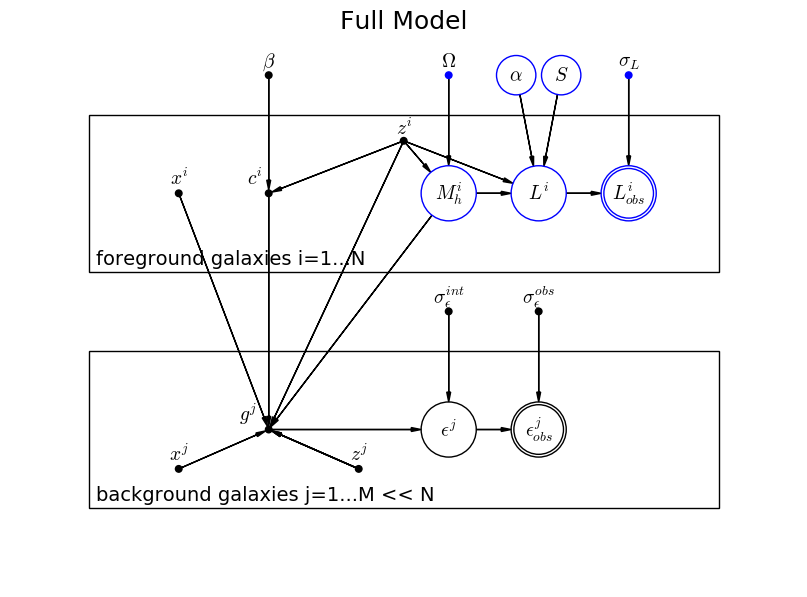
\includegraphics[width=2.0\columnwidth]{full_pgm.png}
\caption{
Above is a probabilistic graphical model for the full model we aspire to. 
There are two plates; one for foreground galaxies, one for background galaxies. 
The cosmology hyperparameters are colored green, the mass luminosity relation hyperparameters are colored blue, and the noise hyperparameters are colored red.
Below is a table with all the parameters and corresponding descriptions.
\label{fig:ultimate_pgm}}
% \end{figure}

% \begin{table*}[h]
\begin{center}
\begin{tabular}{|c|l|}
\hline
Parameter & Description\\ 
\hline
$\beta$ & Form of the halo concentration.\\
$\Omega$ & Cosmology used to generate the halos in the Millennium Simulation.\\
$\alpha$ & Four parameters that convert mass to mean luminosity.\\
$S$ & Scatter of the mass luminosity relationship.\\
$M$ & Halo mass.\\
$L$ & Galaxy luminosity.\\
$x$ & Angular position of galaxy.\\
$z$ & Galaxy redshift.\\
$c$ & Halo concentration.\\
$g$ & Reduced shear.\\
$\epsilon$ & Galaxy shear.\\
$\sigma$ & Various forms of noise.\\
\hline
\end{tabular}
\end{center}
\end{table}

The model partitions galaxies into two groups. 
Background galaxies are sources that lie in a redshift bin immediately behind the three dimensional space of foreground galaxies. 
The background galaxies provide the observed shears which we use to infer the halo masses of foreground galaxies. 
We plan to use around 200,000 foreground galaxies and 1,600 background galaxies in our model and analysis. 
In the course of the heirarchical inference, each of the 200,000 galaxies contributes and has a corresponding mass and luminosity which must be marginalized out. 
Given the large size of our inference, we expect the primary challenges to be computational in nature - how can we achieve inference at this unprecedent scale?
In order for us to rapidly iterate towards an answer to this question, we study a model with simpler dependencies.
This condensed model, shown in Figure \ref{fig:simplified_pgm}, offers the benefit of being easier to test while retaining the computational challenges that need to be adressed.

\begin{figure}[h]
\centering
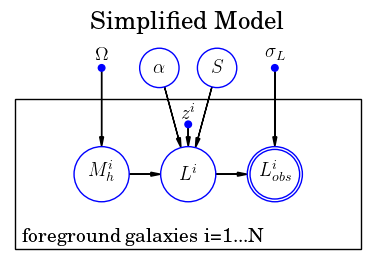
\includegraphics[width=0.9\columnwidth]{try2.png}
\caption{
A probabilistic graphical model for the simplified model we will use for testing.
The parameters are a subset of those in Figure \ref{fig:ultimate_pgm}.
\label{fig:simplified_pgm}}
\end{figure}

The data we use is derived from the Millennium Simulation \citep{millennium}. 
Our selection is driven by our desire to incorporate weak lensing into our ultimate model, which necessitates the large number of halos. 
Furthermore, \citet{raytracing} have also performed raytracing on this dataset which we plan to make use of in our weak lensing inference. 
There are two transformations that are applied on top of the simulation output.
First, a friend-of-friend (FoF) group finding algorithm identifies halos from the particle concentrations in the simulation output. Second, a $40 \times 40$ square arcminute window of sky out to redshift 3.5 is carved out from the output. 
The interior halos form the foreground galaxies in our analysis.  
The resulting dataset consists of 115,919 halos with accompanying positions (right-ascension, declination, and redshift).

The statistical inference we perform follows the canonical inference formula: posterior equals prior times likelihood. 
In the analysis that follows we use an overline, such as $\overline{z}$, to distinguish a vector over all foreground galaxies from the variable corresponding to a single halo, or $z$.
Given the mass luminosity hyperparameters $\alpha$, $S$; a vector of observed luminosities $\overline{L^{obs}}$; a vector of redshifts $\overline{z}$; and the observational noise in luminosity measurements $\sigma_L^{obs}$ - the posterior we seek is
$$\underbrace{P(\alpha, S| \overline{L^{obs}}, \overline{z}, \sigma_L^{obs})}_{
	\text{Posterior}} = 
\underbrace{P(\alpha, S)}_{\text{Prior}} \underbrace{P(\overline{L^{obs}}| \alpha, S, \overline{z}, \sigma_L^{obs})}_{\text{Likelihood}}$$

Using the probabilistic graphical model we can further factor this to

\begin{align*}P(\alpha, S| \overline{L^{obs}}, \overline{z}, \sigma_L^{obs}) &= P(\alpha)P(S) \\
 \iint \overline{dM}\ \overline{dL}\ &P(\overline{L^{obs}}| L, \sigma_L^{obs}) P(\overline{L}|\overline{M},\alpha,S,\overline{z})P(\overline{M}|\overline{z})
\end{align*}

The likelihood integral involves integrating over 200,000 variables - the mass and luminosity for each galaxy in our dataset. 
The Methods section of this paper describes various approaches to make such a high dimensional integral computationally tractable. 

The integrand of the likelihood contains three probabilities. 
The first is the conditional observed luminosity probability. 
Since luminosities are usually reporeted in log-space, we assume that there are gaussian errors in the log-space luminosity measurements, or that the distribution is log-normal. 
We believe 5\% errors seem reasonable and fix $\sigma_L^{obs} = 0.05$. Our conditional distribution is 

$$P(\overline{L^{obs}}| \overline{L}, \sigma_L^{obs}) = \frac{1}{\overline{L^{obs}}\sigma_L^{obs}\sqrt{2\pi}}\exp\left(-\frac{(\ln \overline{L^{obs}} - \ln \overline{L})^2}{2\sigma_L^{obs\ 2}}\right)$$

The second factor in the likelihood integrand is the mass luminosity relation $P(\overline{L}|\overline{M},\alpha,S,\overline{z})$. 
We use the form described in \cite{reddick}. 
Reddick follows the convention from previous work where the conditional luminosities is divided into two parts, central and satellite galaxy contributions. 
The central contribution is described by a lognormal distribution and the satellite contribution is described by a Schechter function. 
In our analysis, we ignore the satellite contribution. 
This decision is made for convenience, and we can easily insert the satellite contribution in future analyses. 
We use $\alpha = (\alpha_1, \alpha_2, \alpha_3, \alpha_4)$ to represent the parameters for computing the mean luminosity and $S$ for the scatter. 
This gives

\begin{align*}
P(\overline{L}|\overline{M},\alpha,S,\overline{z}) &= \frac{1}{\overline{L}S\sqrt{2\pi}}\exp\left(-\frac{(\ln \overline{L} - \ln \overline{\mu_L})^2}{2S^{2}}\right)\\
\mu_L &= \exp(\alpha_1) \cdot \left(\frac{M}{\alpha_3}\right)^{\alpha_2} \cdot (1+z)^{\alpha_4}\\
\end{align*}

The third factor in the likelihood integrand is the halo mass function $P(\overline{M}|\overline{z})$. 
For this we rely on the python software package \emph{hmfcalc} \citep*{hmf}. 
In the API we select the functional form from \citep{tinker} and the cosmology from the Millennium Simulation to govern the mass function. 
The API returns 400 logarithmically spaced mass samples and the derivative of the number density $\frac{dn}{dM}$. 
We convert this into a probability density with trapezoidal integration.
The function also has a dependence on redshift, which we account for by employing 20 redshift bins and matching the halos in the different redshift bins with the corresponding prior.
Figure \ref{fig:priors} shows the priors for each redshift bin.

\begin{figure}[h]
\centering
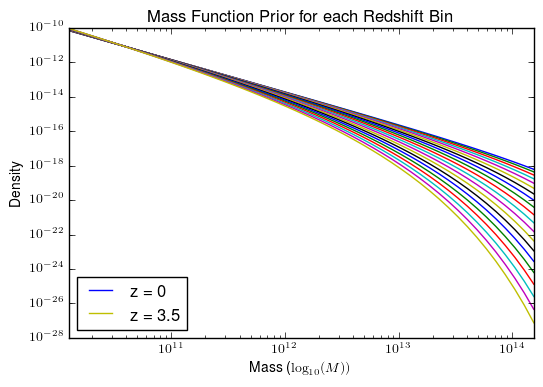
\includegraphics[width=1.0\columnwidth]{priors.png}
\caption{
The mass function prior for the range of redshift bins from z = 0 to z = 3.5.
\label{fig:priors}}
\end{figure}

In Subsection \ref{subsec:epsilon_back} we discuss further modifications to the prior that allow it to work in concert with both sampling and logarithms. 


% ----------------------------------------------------------------------

\section{Methods}
\label{sec:methods}

The critical challenge of the inference is computing the high dimensional likelihood.
In this section we describe the test dataset used in the inference and four different methods for computing the high dimensional likelihood. 

\subsection{Test Dataset}
\label{subsec:testdata}

The scaffold for the test dataset is the catalogue of dark matter halos from \citealt{raytracing}.
This scaffold provides the redshift and mass of each halo.
We augment this initial dataset with a luminosity and observed luminosity for each halo.
In order to do this we need to use the mass luminosity relation which requires the aforementioned set of hyperparameters $\alpha_1, \alpha_2, \alpha_3, \alpha_4, S$. 
We draw a set of hyperparameters from the distributions suggested in \citet{reddick} and fix it for the entire dataset.
Then we use this fixed set of hyperparameters and the mass luminosity relation to generate luminosities for each halo.
Then the noise model is used to generate observed luminosities for each halo.

After testing various methods for computing the likelihood, we can use the dataset to do a complete test of the inference. 
The inference only consumes the redshift and observed luminosity fields of the dataset and produces a hyperparameter posterior.
This posterior can then be compared against the fixed set of hyperparameters that generated the dataset. 
If the process produces posteriors consistent with the fixed values then we can be confident that it will also be able to provide accurate hyperparameter posteriors for real datasets. 

\begin{figure}[h]
\centering
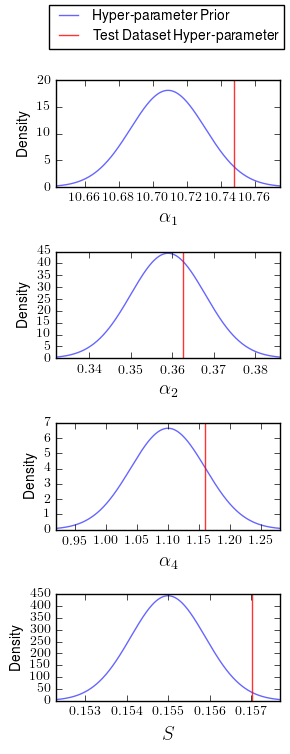
\includegraphics[width=0.95\columnwidth]{drawn.png}
\caption{
The hyperparameter prior is shown in blue and the drawn hyperparameter value for the test dataset is shown in red.
\label{fig:drawn}}
\end{figure}


The original likelihood integral can be factored into a product of integrals corresponding to each halo. Moving forward in this section, we use the convenient substitutions

\begin{align*}
P_1 &= P(L^{obs}|L, \sigma_L^{obs})\\
P_2 &= P(L|M, \alpha, S, z)\\
P_3 &= P(M|z)\\
\end{align*}

\nonident Then letting $D$ be the dataset of halos we have

\begin{align*}
\mathcal{L}(\overline{L^{obs}}|\alpha, S, \sigma_L^{obs}, \overline{z}) &= \prod_{(L^{obs}, z) \in \text{D}}\mathcal{L}(L^{obs}|\alpha, S, \sigma_L^{obs}, z)\\
&= \prod_{(L^{obs}, z) \in \text{D}}\int dMdL\ P_1P_2P_3\\
\end{align*}

Initially, we narrow our focus to a single one of these integrals. 
After we characterize the tradeoffs in the single integral case we expand our analysis to computations of the entire product of integrals. 

\subsection{Numerical Integration}
\label{subsec:numint}

Numerical integration is the canonical way to approximate a continuous integral on a computer.
The domain of integration is partitioned into small rectangles.
Then the integrand is evaluated at the center of each rectangle and multiplied by the surrounding rectangle's area to approximate.
This approximates the true region under the curve over the rectangle.
Summing up the contributions from all the rectangles in the domain provides an approximation of the entire integral.

The precision can be sensitive to the partitioning of the domain. 
Smaller rectangles around a point will provide more precise approximations. 
By increasing the number of rectangles in the partition, and decreasing their area, one can expect to achieve a more precise approximation of the integral.
The partitioning in the mass dimension is somewhat limited by our prior, which is comprised of a normalized, linear approximation on the 410 mass values provided by \emph{hmfcalc}.
Breaking the mass up into more than 410 pieces would increase our reliance on the linear approximation of our prior when computing the integrand, which limits its benefit.
In our implementation we fix the mass partitioning to be the same 410 masses provided by \emph{hmfcalc}.
The runtime is $O(mn)$ where $m$ is the number of mass partitions and $n$ is the number of luminosity partitions.
In our experiments we found the scale of the luminosity partition, linear or logarithmic, to have limited impact on the result and have chosen to stick with logarithmic for slightly improved accuracy when $n$ is small.
Letting $X$ and $Y$ be the logarithmically spaced ranges of $M$ and $L$ respectively, gives

\begin{align*}
\mathcal{L}(L^{obs}|\alpha, S, \sigma_L^{obs}, z) &= \int dMdL\ P_1P_2P_3\\
&\approx \sum_{L \in X}\sum_{M \in Y} \Delta_L\Delta_M\ P_1P_2P_3\\
\end{align*}

Most of the contribution to the value of the integral comes from a small region in the domain. 
Intuition suggests that if we were able to selectively sample from this region we would be able to compute the integral more efficiently. 
This line of thought leads us to simple monte carlo integration.


\subsection{Simple Monte Carlo}
\label{subsec:smc}

Simple monte carlo integration is a method for computing an integral when the variables of integration are probabilities in the integrand.
We can approximate the integral over the probability distribution with samples from the distribution. 
In our likelihood, we employ this approximation for both the conditional luminosity $P(L|M, \alpha, S, z)$ and the prior $P(M|z)$. With these modifications our integral becomes

\begin{align*}
\mathcal{L}(L^{obs}|\alpha, S, \sigma_L^{obs},z) &= \iint dLdM P_1P_2P_3\\
&\approx \frac{1}{N_s}\sum_{L \sim\ P_2}\sum_{M \sim\ P_3} P_1\\
\end{align*}

This joint sampling generates samples with larger products $P(L|M, \alpha, S, z)P(M|z)$.
It could be that the remaining factors in the integrands, $P(L^{obs}|L, \sigma_L^{obs})$, have low weights and mitigate the benefits of this sampling.
This would happen if a halo has an outlier observed luminosity and is not sampling nearby luminosities.
Our setup is particularly prone to this because of the major disparity between the distributions for the mass function prior and the masses of the dataset in the high mass region. 
This suggests that this approach may not be able to accurately compute the likelihood for halos with large observed luminosities.

\subsection{Importance Sampling}
\label{subsec:is}

Consider the rare halo with exceptionally large observed luminosity. 
Simple monte carlo will generate many low mass, low luminosity samples and rarely sample the high weight region of the likelihood integral. 
The sampling would be more efficient if the scheme could adjust its sampling to accomodate the large observed luminosity.
Importance sampling is a statistical technique that makes such strategic sampling possible without altering the result. 

The basic idea behind importance sampling is multiplying the integrand by $1 = Q/Q$, where $Q$ is a strategically designed distribution, which is also nonzero over the domain of integration.
Then instead of sampling from the original distribution $P$, the technique samples from $Q$ and weighs the samples by $P/Q$.
For example, if the simple monte carlo integral is $\int dx\ P(x) = \int dP(x)$, then the importance sampling integral is $\int dx\ \frac{P(x)Q(x)}{Q(x)} = \int dQ(x)\ \frac{P(x)}{Q(x)}$.
A powerful property of importance sampling is that is an unbiased estimator (Appendix \ref{subsec:is_unbiased} contains the proof).
This guarantee gives us the freedom to design a biased distribution $Q$ to generate efficient samples for our likelihood integral. 
To get the most efficient sampling, we strive to develop a biased distribution $Q$ that samples the `important' region where the weights $P/Q$ are high.

Recall that both the conditional luminosity and conditional observed luminosity relations are lognormal.
Given an observed luminosity, we can reverse the lognormal, keeping the same mean, to generate an approximate distribution of luminosities.
For example, to get $L^{obs}$ from $L$ we would take samples from the integrand factor $P(L^{obs}| L, \sigma_L^{obs})$.
To get an approximation of $L$ from $L^{obs}$ we can use 

$$Q(L|L^{obs}, \sigma_L^{obs}) = \frac{1}{L\sigma_L^{obs}\sqrt{2\pi}}\exp\left(-\frac{(\ln L - \ln L^{obs})^2}{2\sigma_L^{obs\ 2}}\right)$$

Similarly, to get an approximation of $M$ from $L$ we reverse the conditional luminosity relation, and reverse the corresponding mean mass luminosity relation as well.

\begin{align*}
Q(M|L,\alpha,S,z) &= \frac{1}{MS_Q\sqrt{2\pi}}\exp\left(-\frac{(\ln M - \ln \mu_M)^2}{2S_Q^{2}}\right)\\
\mu_M &= \alpha_3 \left(\frac{L}{\exp(\alpha_1)(1+z)^{\alpha_4}}\right)^{1/\alpha_2}\\
\end{align*}

The reader may notice how on the right hand side of the first equation above we have replaced $S$ with $S_Q$. 
This is because we use $S_Q = \lambda \cdot S$, where $\lambda$ is the constant which converts the scatter in conditional luminosity to the scatter in conditional mass.
We derive $\lambda$ through an error propagation technique described further in Appendix \ref{subsec:error_prop}.

For convenient notation we let

\begin{align*}
Q_1 &= Q(L|L^{obs}, \sigma_L^{obs})\\
Q_2 &= Q(M|L,\alpha, S, z)\\
\end{align*}

\noindent Combining the above distributions into a joint biased distribution for importance sampling yields the formula below for the single halo likelihood integral.

\begin{align*}
\mathcal{L}(L^{obs}|\alpha, S, \sigma_L^{obs}, z) &= \iint dLdM \frac{P_1P_2P_3Q_1Q_2}{Q_1Q_2}\\
&= \frac{1}{N_s}\sum_{L \sim Q_1}\sum_{M \sim Q_2} \frac{P_1P_2P_3}{Q_1Q_2}\\
\end{align*}


To validate the effectiveness of the biased joint distributions (the Q's) we generate nine different test datasets. For each dataset, hyperparameters are drawn from the prior distribution (defined in Subsection \ref{subsec:testdata}), and used to generate a mass, luminosity, and observed luminosity for each halo in the catalogue.
Then we generate samples from the joint distribution via simple monte carlo and importance sampling and compare how efficiently the two approaches cover the true joint distribution.
Figure \ref{fig:isworks} shows the nine corresponding scatterplots of the first 1,000 samples in the mass and luminosity dimensions. 
As expected, simple monte carlo has poor coverage of the the high mass, high luminosity region.
Importance sampling has much better coverage.

\begin{figure*}[h!]
\centering
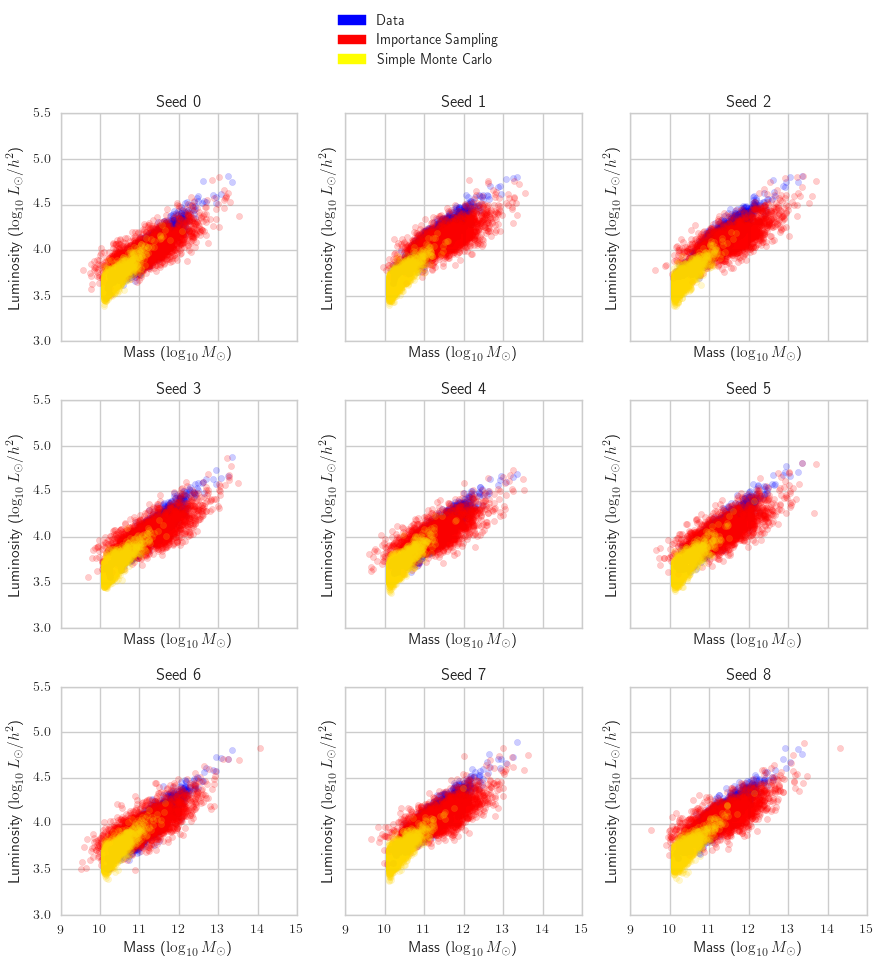
\includegraphics[width=2.0\columnwidth]{isworks.png}
\caption{
Each seed corresponds to a different draw of hyperparameter values. The true joint distribution from the test dataset is in blue, the importance sampling sampling distribution is in red, and the simple monte carlo sampling distribution is in yellow.
\label{fig:isworks}}
\end{figure}

\subsection{Laplace Approximation}
\label{subsec:laplace}

The final scheme we explore adheres to paradigms from optimization. 
In this paradigm we view the integrand as a smooth surface with a hill that corresponds to the high weight, or important region of the integrand. 
To compute the integral we iteratively hike up the landscape to the highest point on the hill, the maximum of the integrand. 
From this vantage point we approximate the hill with an easy-to-integrate multivariate distribution centered on the maximum. 
The integral of the distribution serves as a rough approximation of the original integral.

To find the maximum of the integrand we use the Broyden-Fletcher-Goldfarb-Shanno (BFGS) method implemented in \emph{scipy.stats.minimize} \citep{scipy}. 
We pass the negative-log-integrand, $-\ln I(M,L)$, to the optimizer which returns the optimal point $(M^{opt}, L^{opt})$ and the inverse hessian matrix $H^{opt\ -1}$ at the optimum. 
We then approximate the integrand as 

\begin{align*}
I^*(M,L) &= I(M^{opt}, L^{opt})\exp\left(\frac{v^TH^{opt}v}{2}\right)\\
v &= (M,L) - (M^{opt}, L^{opt})\\
\end{align*}

\noindent which has the closed form integral 

$$\iint dMdL\ I^*(M,L) = \sqrt{\frac{4\pi^2}{\det(H^{opt})}}$$

\noindent In practice we must also apply a numerical trick to produce satisfactory inverse hessian matrices from the optimizer. Appendix \ref{subsec:rescale_la} describes this technique in detail.

% ----------------------------------------------------------------------

\section{Results}
\label{sec:results}

We start by examining the behavior of the four methods in the context of a single halo. Next we scale two of the methods to run over a field of view with multiple halos. Then we analyze the accuracy and show the results from the full inference.

\subsection{Single Halo Likelihood}
\label{subsec:single_halo}

The key difference between the four likelihood integration methods described in Section \ref{sec:methods} is how they marginalize over the masses and luminosities of the halos. 
To see these differences more clearly we narrow the scope of the likelihood function to a single halo evaluated on a fixed set of hyperparameters.
Each single likelihood of a halo is dependent on the halo to which it corresponds.
To get a sense of how the single halo likelihoods vary across the halos in our dataset, we create a test suite of four halos (Halo 0, Halo 1, Halo 2, Halo 3).
The test halos are a combination of boring representative halos and outlier halos which we anticipate will further expose key differences.
Halo 0 comes from a moderately probable part of the joint distribution; Halo 1 is an outlier with low mass and luminosity, Halo 2 is close to the peak of the distribution; Halo 3 is an outlier with high mass and luminosity.  
Figure \ref{fig:joint} shows the joint mass and luminosity distribution of the entire dataset and the test halos we have chosen.

\begin{figure}[!h]
\centering
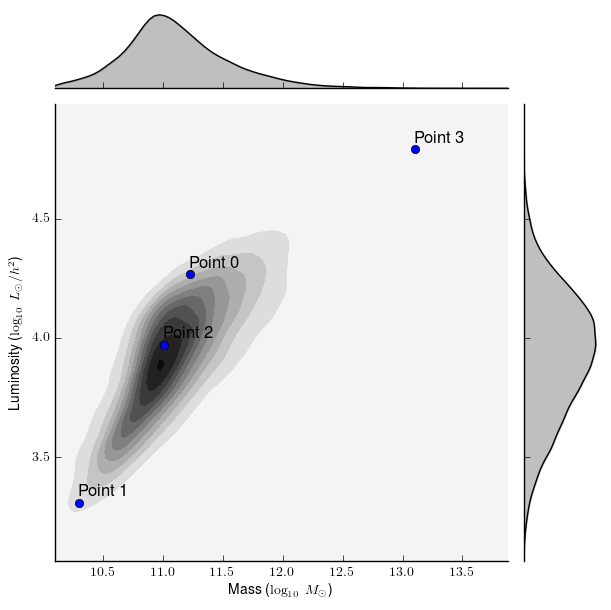
\includegraphics[width=1.0\columnwidth]{joint.png}
\caption{
The mass and luminosity joint distribution from the test dataset is shown in violet and the four chosen test halos are shown in red. 
\label{fig:joint}}
\end{figure}

For each test halo we compute the likelihood by four methods: numerical integration, simple monte carlo, importance sampling, and laplace approximation. The result and a breakdown of the techniques is shown in Figure \ref{fig:points} and its companion Table \ref{tab:points}.

The column of numerical integration plots in Figure \ref{fig:points} shows the technique attains solid coverage of the domain and suggests that this method be the most accurate. 
Since the mass prior drops precipitously outside the displayed mass range, it is safe to assume that even for the numerical integration for Halo 1 which appears cutoff in the figure, the technique still contains the contributing region.
We use numerical integration as an answer key that we from which we judge the accuracy of other methods. 

\begin{figure*}[h]
\centering
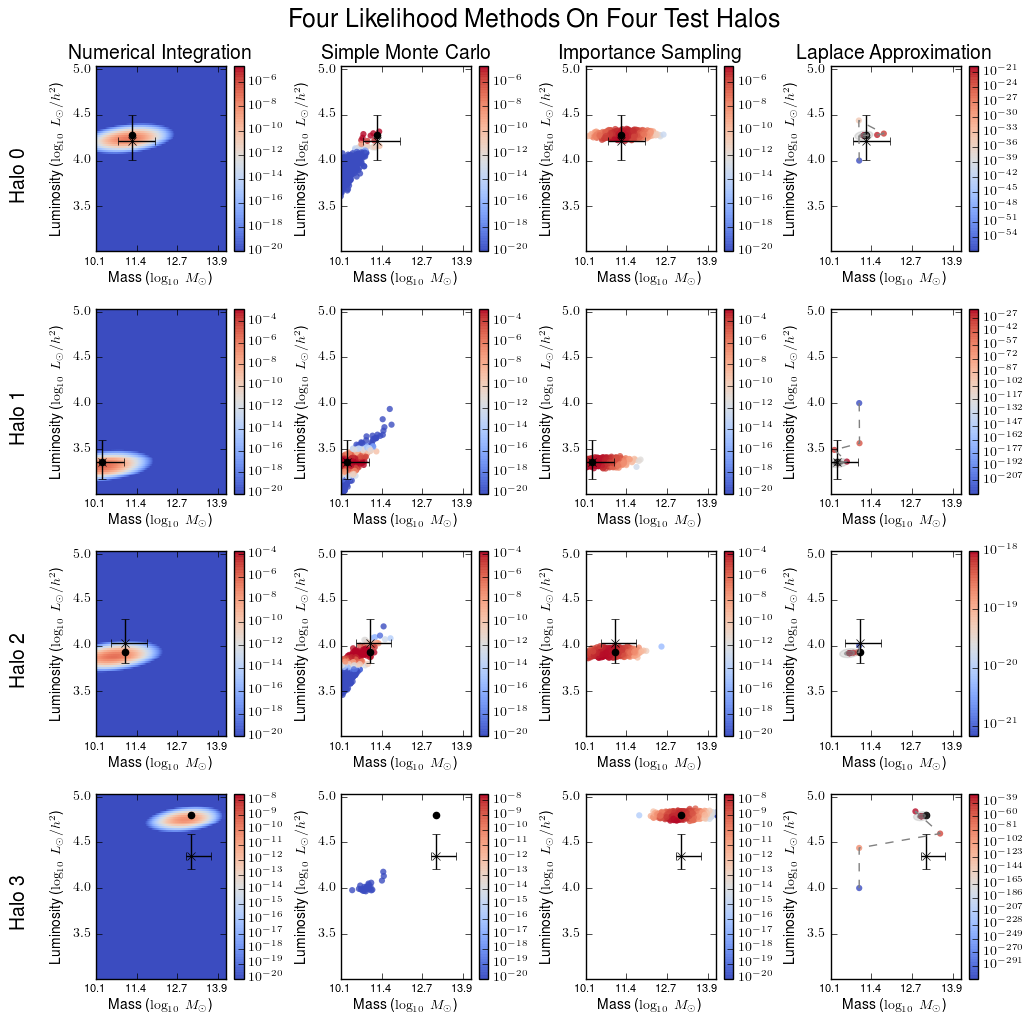
\includegraphics[width=2.0\columnwidth]{points.png}

\caption{
An array of plots characterizing how the different methods marginalize the mass and luminosity joint distribution for the different test halos.
Each row corresponds to one of the different test halos.
Each columns corresponds to one of the different methods.
All plots have the same axes and the plots in the first three columns have the same color weight scale.
Each of the first three plots is a scatter plot of the samples taken by the corresponding method colored according to their contribution to the likelihood.
Red samples contribute heavily; blue samples contribute lightly.
The black dot is the true mass and luminosity of the test halo and the black bars are the $2\sigma$ error bars for the joint distribution.
The fourth column contains a scatter plot of the points generated in the iterative optimization method, with sequential points connected by a gray dashed line.
The resulting multivariate normal distribution's $1\sigma$ and $2\sigma$ are in light gray. Table \ref{tab:points} shows the likelihood values corresponding to these plots.
\label{fig:points}}

% Let's step through the panel in Figure \ref{fig:point1} which corresponds to Point 0.
% The plot corresponding to Numerical Integration is in the upper right.
% The black dot is the true mass and luminosity of the halo whose likelihood we are computing.
% The nearby black band shows the mean and standard deviation of the luminosity distribution from our test dataset, conditioned on both mass and redshift bins.
% This helps us understand whether the likelihood halo is an outlier.
% The points of the plot are the halos sampled by the method.
% For the laplace approximation we use the optimal point after each iteration as the set of samples.
% The light gray dotted line between them shows the order of the optimal path. 
% The two ovals around the optimal point are the 1$\sigma$ and 2$\sigma$ epigraphs of the laplace approximation multivariate gaussian.
% The color of the point shows the \emph{weight} it contributes to the likelihood.
% In numerical integration and laplace approximation the weight is the original integrand $P(L^{obs}|L, \sigma_L^{obs})P(L|M, \alpha, S, z)P(M|z)$.
% In simple monte carlo and importance sampling, we use the concept of \emph{weight} to distinguish from the probability density functions in the numerator that are used to generate samples from the ones that are evaluated and contribute to the sum.
% In simple monte carlo the weight is $P(L^{obs}|L, \sigma_L^{obs})$ and in importance sampling the weight is $\frac{P(L^{obs}|L, \sigma_L^{obs})P(L|M, \alpha, S, z)P(M|z)}{Q(L|L^{obs}, \sigma_L^{obs})Q(M|L,\alpha, S, z)}$.
% The different weight functions have different ranges.
% To increase the informativeness of the panel we cap the weights for numerical integration, simple monte carlo, and importance sampling from below at $10^{-20}$. 
% \label{fig:points}}
\end{figure*}

\begin{table}[h]
\centering
\begin{tabular}{|l|r|r|r|r|}
\hline
Test Halo & Halo 0\\
\hline
Numerical Integration & 6.40358058377 \times 10^{-06}\\
Simple Monte Carlo & 8.57179497702 \times 10 ^{-07}\\
Importance Sampling & 6.39959705909e \times 10 ^{-06}\\
Laplace Approximation & 3.68701955823e \times 10 ^{-06}\\
\hline
Test Halo & Halo 1\\
\hline
Numerical Integration & 0.000487808661776\\
Simple Monte Carlo & 0.000487547191603\\
Importance Sampling & 0.000487206370881\\
Laplace Approximation & 0.000316487709918\\
\hline
Test Halo & Halo 2\\
\hline
Numerical Integration & 6.27613065943e-05\\
Simple Monte Carlo & 2.82394491619e-05\\
Importance Sampling & 6.29604927168e-05\\
Laplace Approximation & 3.80374065466e-05\\
\hline
Test Halo & Halo 3\\
\hline
Numerical Integration & 5.57536196939e-09\\
Simple Monte Carlo & 3.49945536295e-53\\
Importance Sampling & 5.57880154767e-09\\
Laplace Approximation & 2.89024212204e-09\\
\hline
\end{tabular}
\caption{
Companion table to Figure \ref{fig:points}. Contains the single halo likelihood value for each of the test halos (rows) under the different methods (columns).
\label{tab:points}}
\end{table}

% \begin{table}[h]
% \centering
% \begin{tabular}{|l|r|r|r|r|}
% \hline
% Test Halo & Numerical Integration & Simple Monte Carlo\\
% \hline
% Halo 0 & 6.40358058377e-06 & 8.57179497702e-07\\
% Halo 1 & 0.000487808661776 & 0.000487547191603\\
% Halo 2 & 6.27613065943e-05 & 2.82394491619e-05\\
% Halo 3 & 5.57536196939e-09 & 3.49945536295e-53\\
% \hline
% Test Halo & Importance Sampling & Laplace Approximation\\
% \hline
% Halo 0 & 6.39959705909e-06 & 3.68701955823e-06\\
% Halo 1 & 0.000487206370881 & 0.000316487709918\\
% Halo 2 & 6.29604927168e-05 & 3.80374065466e-05\\
% Halo 3 & 5.57880154767e-09 & 2.89024212204e-09\\
% \hline
% \end{tabular}
% \caption{
% Companion table to Figure \ref{fig:points}. Contains the single halo likelihood value for each of the test halos (rows) under the different methods (columns).
% \label{tab:points}}
% \end{table}

Simple monte carlo generates a narrow, diagonal slice of samples, which is consistent with the conditional luminosity relation.
Halo 3 shows how terribly suited this approach is for outlier halo likelihoods.
Even for Halos 1 and 2 where it produces some high weight samples, it misses out on capturing the true oval shape of the high weight region.
While this approach has attractive computational aspects, its inefficient sampling, fully exposed by outliers, renders it completely unsatisfactory for our purposes.

Importance sampling is an attractive remedy to the problems that plague simple monte carlo.
Almost all the samples are high weight and the oval nature of the high weight region is captured.
Even for the outlier Halo 3, this technique performs very well.
It is also encouraging that the likelihood values produces from this technique are in great agreement with the values from numerical integration.

Both simple monte carlo and importance sampling are sampling techniques; we can use effective sample size to compare their sampling efficiencies (further described in Appendix \ref{subsec:is_ess}).
The effective sample size is roughly the number of samples which are contributing to the estimate in a nontrivial manner.
Figure \ref{fig:table} shows the effective sample sizes for the four points for both sampling methods. The exceptionally low values for $n_{eff}^{SMC}$ show that simple monte carlo is unreliable, especially on the outlier Halo 3.
Importance sampling however, is both efficient, $n_{eff}^{IS} \approx n/2$, and consistent, $n_{eff}^{IS}$ is similar for different points, even on the outliers.
The extreme difference between $n_{eff}^{SMC}$ and $n_{eff}^{IS}$ reinforces that importance sampling is a dramatic improvement over simple monte carlo and suggests this improvement is necessary to sample the likelihood effectively.

\begin{table}
\begin{center}
\begin{tabular}{|c|c|c|}
\hline
Test Halo & $n_{eff}^{SMC}$ & $n_{eff}^{IS}$\\ 
\hline
Halo 0 & $3$ & $624$\\
Halo 1 & $191$ & $562$\\
Halo 2 & $45$ & $619$\\
Halo 3 & $1$ & $518$\\
\hline
\end{tabular}
\end{center}
\caption{For each of the four test halos we compare the effective sample size of simple monte carlo $n_{eff}^{SMC}$ to the effective sample size of importance sampling $n_{eff}^{IS}$, both with 1000 samples.}
\label{fig:table}
\end{table}

The laplace approximation is a different approach entirely.
We see that the optimization finds the optimal point quickly, getting to within 0.1 distance within a handful of iterations.
But the hessian and the multivariate normal distribution it produces are a bit small.
This visual intuition from Figure \ref{fig:points} is confirmed by the consistent laplace approximation underestimation seen in Table \ref{tab:points}.
The laplace approximation solutions are smaller than the solutions from numerical integration and importance sampling by a factor hovering around two.
The estimate may be sensitive to the form of the approximating distribution.
The sensitivity may be explored in future work.

The goal of pursuing alternative likelihood computation methods is to achieve an accurate answer with lower computational costs. 
The cost is related to sampling efficiency, but there are other factors that contribute.
Figure \ref{fig:convergence} shows the likelihood convergence and runtime for Halo 0 versus the number of samples used in the method for our Python implementation of these methods (Appendix \ref{subsec:code}).
Since the laplace approximation is not a sampling technique, and does not have number of samples as a parameter, it is approximately constant in both plots. 


\begin{figure}[!h]
\centering
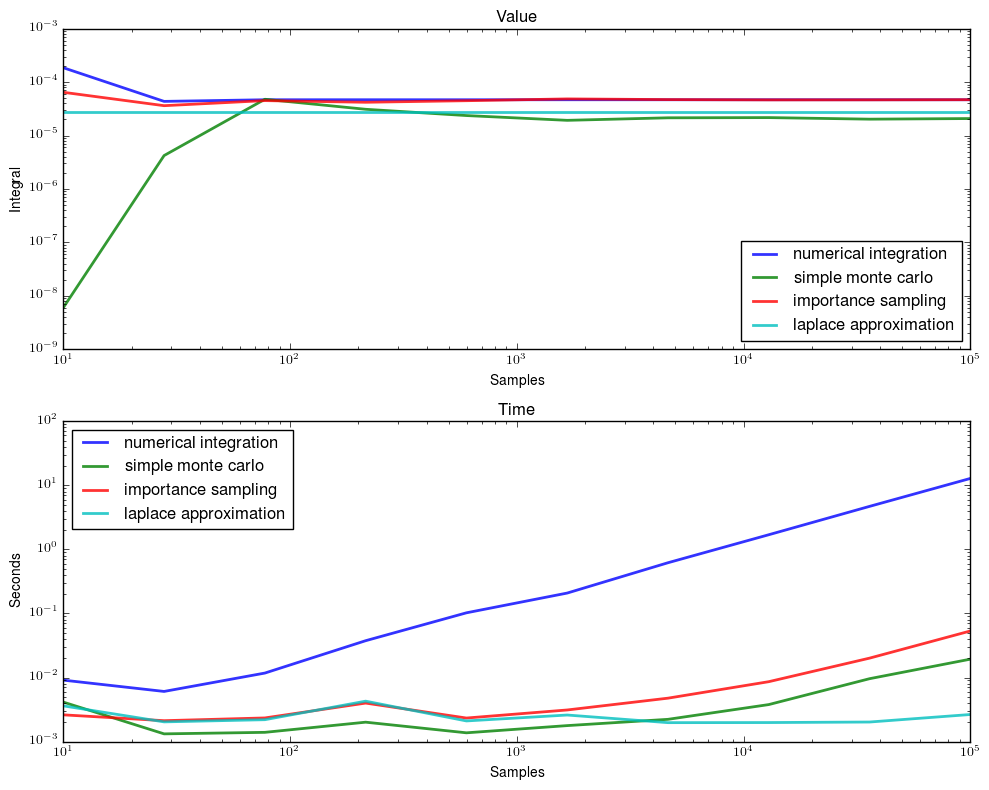
\includegraphics[width=0.9\columnwidth]{convergence.png}
\caption{
Top panel: the likelihood value for Halo 0 for varying numbers of samples.
Bottom panel: the Python implementation runtime of the likelihood computation for varying numbers of samples.
\label{fig:convergence}}
\end{figure}

The convergence plot in Figure \ref{fig:convergence} confirms our suspicions from Figure \ref{fig:points}.
Simple monte carlo is widely inaccurate and differs by numerical integration by over an order of magnitude. 
Even with many samples this method exhibits instability.
The laplace approximation is an improvement, but underpredicts by about a factor of two.
If this underprediction is consistent across posterior samples then the technique may be salvageable. 
Importance sampling and numerical integration are more promising. 
Both converge to stable values rapidly and are in remarkable agreement.
These patterns remain when we switch the likelihood to different halos.

The runtime plot in Figure \ref{fig:convergence} shows that numerical integration, importance sampling and simple monte carlo have constant runtimes initially and transition to linear runtime. 
Our software profiling confirms that this is due to the fixed memory allocation cost dominating for small sample sizes and cpu processing dominating for larger sample sizes.
The cpu time dominates sooner in numerical integration because of the large grid of computations it makes.
It is also worth recalling that the number of mass values used in numerical integration is constant while the number of luminosity samples is a parameter.
This is why the runtime grows linearly with the number of samples as opposed to quadratically.
Numerical integration takes $\sim 10^3$ times longer than simple monte carlo. Fortunately, importance sampling only takes $\sim 2$ times longer and the laplace approximation has constant runtime in theory.

Given the strict grid sampling of numerical integration, we expect it to be the most accurate likelihood method.
While we cannot compare this approximation method to a closed form solution for the problem, we can test its self consistency.
As the number of samples increases, the sampling resolution improves, which should improve the accuracy in turn.
Table \ref{tab:ni_acc} shows the numerical integration values for the four test halos at varying numbers of samples.
The likelihood value gains two digits of precision for each order of magnitude increase in the number of samples from $10^2$ to $10^5$.
Numerical integration is self consistent and achieves significant precision with a small number of samples. We use it to measure the accuracy of the other methods.

\begin{table}[!h]
\centering
\begin{tabular}{|l|r|}%r|r|}
\hline
Samples & Halo 0\\
\hline
100 & \boxed{6.40}23729274 \times 10^{-06}\\
1000 & \boxed{6.4035}688384 \times 10^{-06}\\
10000 & \boxed{6.403580}5837 \times 10^{-06}\\
100000 & \boxed{6.40358070}10 \times 10^{-06}\\
\hline
Samples & Halo 1\\
\hline
100 & \boxed{4.87}71666550 \times 10^{-04}\\
1000 & \boxed{4.8780}776704 \times 10^{-04}\\
10000 & \boxed{4.878086}6177 \times 10^{-04}\\
100000 & \boxed{4.87808670}70 \times 10^{-04}\\
\hline
Samples & Halo 2\\
\hline
100 & \boxed{6.27}49470451 \times 10^{-05}\\
1000 & \boxed{6.2761}191479 \times 10^{-05}\\
10000 & \boxed{6.276130}6594 \times 10^{-05}\\
100000 & \boxed{6.27613077}43 \times 10^{-05}\\
\hline
Samples & Halo 3\\
\hline
100 & \boxed{5.57}43105124 \times 10^{-09}\\
1000 & \boxed{5.5753}517431 \times 10^{-09}\\
10000 & \boxed{5.575361}9693 \times 10^{-09}\\
100000 & \boxed{5.57536207}14 \times 10^{-09}\\
\hline
\end{tabular}
\caption{
Numerical integration values for different numbers of samples (rows) and test halos (columns). The boxed digits are rougly the precision.
\label{tab:ni_acc}}
\end{table}

To measure the accuracy of importance sampling we first get the numerical sampling value and then run importance sampling many times with different random seeds to generate a distribution of results. We repeat this for varying numbers of samples. Figure \ref{fig:is_precision} is the result of this procedure. The relative error is relatively small and decreases with increasing numbers of samples. The $2\sigma$ band is tight, which means importance sampling is fairly stable. The relative error distributions for the different halos are similar and suggest that we may be able to model it as an independent identically distributed random variable.

\begin{figure}[h]
\centering
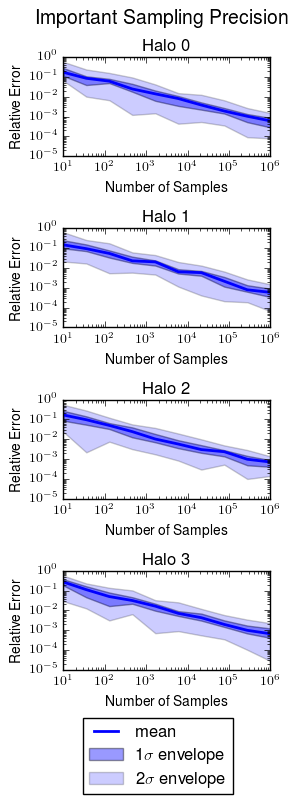
\includegraphics[width=0.8\columnwidth]{is_precision.png}
\caption{
The accuracy of importance sampling against the number of mass and luminosity samples it consumes. The distribution for the 1$\sigma$ and 2$\sigma$ envelopes is generated from the random samples in different importance sampling runs. We use the numerical integration result with 100 samples as the true value for determining accuracy.
\label{fig:is_precision}}
\end{figure}

So far we have been examining the likelihood for a single halo at a fixed set of hyperparameters. We have found that importance sampling closely matches numerical integration and is reasonably stable. Next we examine how these methods perform on different likelihood samples for Halo 0. For each of the four varying hyperparameters, we sample the likelihood along the parameter while holding the others fixed (see Figure \ref{fig:posterior_all}). This provides a rough sense of the shape of the four dimensional likelihood surface. The likelihoods from importance sampling are almost indistinguishable from likelihoods from numerical integration. The laplace approximation likelihood surfaces have the same general shape but are too jagged and erratic to be employed for inference. 

\begin{figure}[!h]
\centering
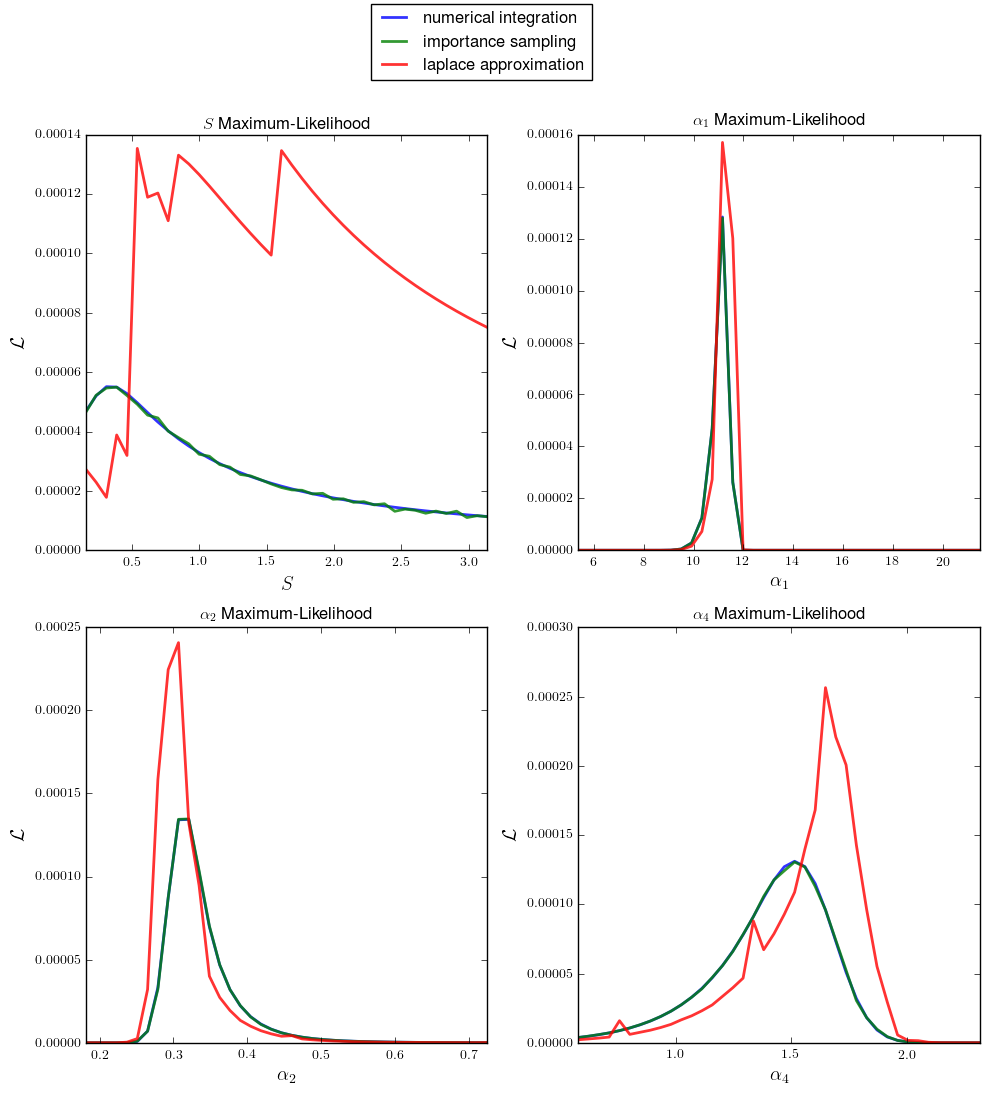
\includegraphics[width=0.8\columnwidth]{posterior_all.png}
\caption{
The single integral likelihood surfaces over lines in hyperparameters $S, \alpha_1, \alpha_2, \alpha_4$. 
\label{fig:posterior_all}}
\end{figure}

This section has exposed key inadequacies of using simple monte carlo or laplace approximation to compute the likelihood. We move forward with only numerical integration and importance sampling as viable methods for the full likelihood.

\subsection{Multiple Halo Likelihood}
\label{subsec:multiple_halos}

In this section we examine critical question: can numerical integration or importance sampling scale to our target of almost 116,000 halos? First we measure runtimes of high performance implementations, then we model errors, and ultimately we highlight our best computation of the posterior.

If the computation scales linearly with the number of halos, then the runtime gets multiplied by a factor of almost 116,000 - making performance critical as we transition from the single halo context to the multiple halo context. We have pursued three different implementations of our methods to attain the best performance. 

The first implementation is a Python implementation with a few enhancements. It heavily relies on the NumPy package and follows the suggested practices in \citealt{numpy}: vectorizing calculations, avoiding copying data in memory, and minimizing operation counts. All objects that can be precomputed or reused are. It also employs a custom implementation of a lognormal evaluation because we have found \emph{scipy.lognorm.pdf} to be an order of magnitude slower, even when called on a scipy.lognorm instance many times (its not just the constructor of the object) \citep*{scipy}. This code has been heavily profiled and we believe offers the best performance we can get from single process Python.

The second implementation is a Python implementation that uses the Numba package to take advantage of its just-in-time (jit) compilation \citep*{numba}. In order to fully take advantage of the jit it is best to have as much of the code as possible as standard Python source code as opposed to invoking external packages. NumPy methods in particular, cannot be tracked and optimized by this method because many of them call native code. We have attempted to exploit the faster \emph{nopython} compilation mode by rewriting much of the original implementation in standard python loops and math operations but there are still a few inconvertible NumPy objects that pollute the jit and prevent us from realizing a speedup. In our experiments, the jit overhead outweighs any improvements to performance.

The third implementation is in C++. We are able to re-use memory more effectively and realize a solid performance improvement. Figure \ref{fig:multi_convergence} shows how the runtimes of these implementations scale with respect to the number of samples and the number of halos. As expected, the C++ implementations are the fastest.

\begin{figure}[!h]
\centering
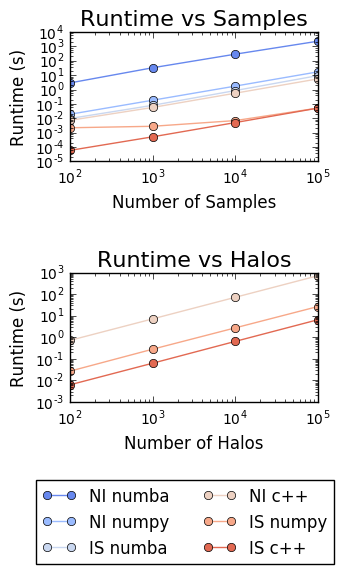
\includegraphics[width=0.9\columnwidth]{multi_convergence.png}
\caption{
Runtimes of the three implementations with respect to the number of samples for one halo (top panel) and the number of halos used with 100 samples (bottom panel).
\label{fig:multi_convergence}}
\end{figure}

We can use Figure \ref{fig:multi_convergence} to extrapolate the runtimes for computing the likelihood on full dataset with almost 116,000 halos. Importance sampling with 100 samples would take approximately 10 seconds;  numerical integration with 100 samples would take approximately 5 minutes.

Presumably there is some error in each of the individual halo likelihoods in the importance sampling approach. Since the total likelihood is a product of many individual halo likelihoods, error may accumulate rapidly. In order to model and constrain the error in this process we collect computationally expensive error statistics on importance sampling's performance on 2\% of the total number of halos, then extrapolate these statistics to predict the error on the total number of halos.

We use a simple model to make error predictions. Let the set of halos be $H$. Then we assume that the log-likelihood corresponding to each halo has an intrinsic true value $v_i$ and a random variable $\epsilon_i$ representing the error. The log-likehood over the entire dataset is then

$$\ell = \sum_{i\in H}\left(v_i + \epsilon_i \right)$$

Now let $H^\prime$ be the subset of 2,000 randomly drawn halos which we will use in our estimate. For each of these halos we extract three parameters: the `true` numerical integration likelihood $n_i$, the standard deviation of the importance sampling likelihoods $\sigma_i$, and the mean difference between the numerical integration and the importance sampling likelihoods $b_i$. Given the precision and stability of numerical integration, we use it as the `true` value of the likelihood, which means $v_i = n_i$. Under this assumption $b_i$ represents the bias in an individual halo likelihood. We also model the individual likelihood errors as normal distributions. Let D(x) be the distribution corresponding to the histogram of samples from $H^\prime$. For example, $D(n_i)$ is the distribution corresponding to $\{n_i\}_{i\in H^\prime}$. Then we can estimate the log-likelihood over the entire dataset as

\begin{align*}
\hat{\ell} &= \sum_{i\in H}\left(n_i^\prime + \epsilon_i^\prime \right)\\
\epsilon_i^\prime &\sim \mathcal{N}(b_i^\prime, \sigma_i^2^\prime)\\
n_i^\prime &\sim D(n_i)\\
b_i^\prime &\sim D(b_i)\\
\sigma_i^\prime &\sim D(\sigma_i)\\
\end{align*}

\noindent Figure \ref{fig:pred_err} shows the predicted and empirical full likelihood distributions. The dispersions of the predicted and empirical likelihood distributions are in great agreement. The standard deviations of the three predicted distributions are 15, 5.1, and 1.7 and the standard deviations of the empirical distributions are 13, 4.8, and 2.3. 

There is a discrepancy between the means of the distributions when plotted on this scale. However, the relative discrepancy is about 0.02\%. In the empirical distributions we see the likelihood slightly increase with the number of samples whereas in the predicted distributions we see it decrease. This is because the true single likelihood noise is not a normal distribution like we assume. Overall, we believe the simple error model does an effective job of representing the full likelihood behavior of importance sampling. 

\begin{figure}[h]
\centering
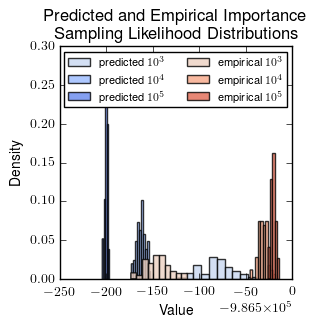
\includegraphics[width=0.9\columnwidth]{pred_err.png}
\caption{
The predicted and empirical distributions for the full likelihood with $10^3, 10^4, 10^5$ samples used for each individual halo. 
\label{fig:pred_err}}
\end{figure}

Todo: Discuss bias, show full likelihood results when computation finishes.

% \section{Discussion}
% \label{sec:discussion}

% \subsection{Interpretation of Single Integral Results}
% \label{subsec:interp}
% We have explored four methods for performing the likelihood corresponding to a single halo and marginalizing over masses and luminosities: numerical integration, simple monte carlo, importance sampling, and laplace approximation. [reiterate tradeoffs]

% If we use a lognormal approximation in the laplace approximation we might better capture the tail of the distribution and produce more accurate approximations. We are interested in searching for a closed form solution of this problem in future work. 

% Reproducibility is an essential feature of science. We encourage others to reproduce our results with the \emph{BigMaLI} python package which can be found on github at \code{https://github.com/davidthomas5412/BigMaLI}.

% High performance computing is essential to our work. We have shaved off a lot of time on the importance sampling by implementing a fastlognorm method which outperforms \emph{scipy.stats.lognorm} sampling by a factor of 10. 

% Another technology we explored is just in time compilation. For this we setup the \emph{numba} python package \citep{numba}. While there are lots of examples of numba accelerating pure python code, it struggles when modules that make calls to c/c++ are used. This is because the interpretter cannot collect runtime stats on these segments of the code. Our code makes heavy use of the \emph{numpy} module, so we measured an increase in runtime when using numba due to its overhead.



% \subsection{Achieving Practical Runtime for Importance Sampling}
% \label{subsec:achieve_runtime}

% While implementing the likelihood codes we have simultaneously been regularly profiling our code. This makes us fairly confident that the current python implementation is about as fast as we can get from single process and thread python code. In importance sampling, each likelihood sample takes around 10 minutes. We expect that the markov chain monte carlo method we use to generate a posterior will require around 10,000 samples. With our current setup this would take seventy days.

% Fortunately, we have many promising leads on how to further accelerate this computation. The first is reducing the number of mass and luminosity samples used in each integral. Figure \ref{fig:is_convergence} shows that we can still achieve decent accuracy with 1,000 samples per halo as opposed to our default of 10,000. This will reduce the runtime by a factor of one third.

% The major bottleneck with our python implementation is the sampling and evaluations where we heavily exploit numpy. Each time numpy methods are called the operating system must allocate new memory. We have implemented lognormal sampling code in python and c++ for comparison. We find that the c++ code, which efficiently reuses memory, is faster by a factor close to 15. By reimplementing our code in c++ we can achieve a 15x speedup and transition from being memory-allocation-bound to CPU-bound.

% Finally, there are great computational resources available at the Stanford National Accelerator Laboratory. The Sherlock batch cluster has over 500 multicore nodes. The MCMC sampling can also be parallelized, increasing throughput close to linearly. Assuming that we can access 1,000 cores by using the Message Passing Interface (MPI), we expect to achieve close to a 1,000 times speedup of our posterior sampling.

% Combining these speedups we find that we can achieve a throughput of 0.04 seconds per sample and complete the entire inference in 5 minutes.




% ----------------------------------------------------------------------

\section{Conclusions}
\label{sec:conclusions}

In this paper we explore four methods for solving a large heirarchical inference: numerical integration, simple monte carlo, importance sampling, and laplace approximation. The inference likelihood is a product of likelihoods for each halo in the field of view. We analyze how our methods perform on an individual halo before scaling numerical integration and importance sampling to the full likelihood. Our conclusions are:

\begin{itemize}
\item Simple monte carlo is not able to sample outliers effectively.
\item Laplace approximation consistently underpredicts the likelihood and produces unstable posterior weights.
\item Importance sampling improves on simple monte carlo by sampling outliers effectively. However, as the number of halos increases, the method accumulates error. Even with $10^5$ samples per each halo likelihood the posterior is dominated by a single sample. 
\item Numerical integration is more computationally expensive than the other methods, but should produce an accurate posterior when $10^4$ samples per halo likelihood are used. We estimate 250,000 core-hours of compute should be enough to produce a reasonable posterior.
\end{itemize}

% We have examined four different methods for computing the likelihood for our inference: numerical integration, simple monte carlo, and importance sampling. We find importance sampling to provide the best combination of accuracy and performance. Furthermore, we have a clear path from lowering the already accelerated likelihood runtime from approximately 10 minutes to 0.04 seconds.


% ----------------------------------------------------------------------

\subsection*{Acknowledgments}

% 
This is the text imported from \code{acknowledgments.tex}, and will be replaced by some standard LSST DESC boilerplate at some point.
% 


\input{contributions}

%{\it Facilities:} \facility{LSST}

% Include both collaboration papers and external citations:
\bibliography{main}

\newpage

\section{Appendix}
\label{sec:appendix}

\subsection{Code}
\label{subsec:code}

Todo. List where code can be found etc.

\subsection{Epsilon Mass Function Background}
\label{subsec:epsilon_back}
Throughout the inference we use logarithms to improve numerical stability.
The \emph{log} function is not defined at zero which creates issues when sample halos are outside the bounds of the mass prior. 
A simple solution is adding a small background probability so that the function is always nonzero. 
There are two further modifications that must be made to make this work. 
First, the prior density must be recomputed so that it integrates to one.
Forgetting to do this leads to nontrivial accumulated errors in the importance sampling.
The second issue is when we sample from the prior we would not like many samples outside the original priors' support.
By making the background probability, which we call $\epsilon$, very small we can ensure that almost all samples are from the mass range of the original prior. 
We set $\epsilon = 10^{-30}$ over the mass range $[10^0, 100 * \text{MaxMass}]$ and renormalize the probability density accordingly.
In expectation, every $\sim 10^{30-18} = 10^{12}$ samples we draw lie outside the original support.
This small number will have negligible impact.
Figure \ref{fig:epsback} shows the updated mass function prior.

\begin{figure}[h]
\centering
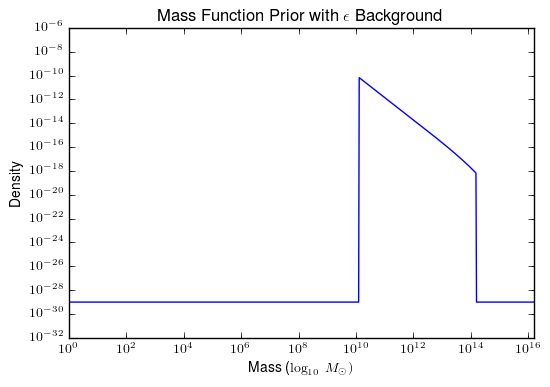
\includegraphics[width=0.6\columnwidth]{epsback.png}
\caption{
The mass function prior for z = 0 over the full range.
\label{fig:epsback}}
\end{figure}

\newpage

\subsection{Importance Sampling Is An Unbiased Estimator}
\label{subsec:is_unbiased}

We prove that in expectation, the mean attained from importance sampling is the true mean of the distribution.
Consider $\mu = \int_D dx\ f(x)p(x)$ where $D$ is the domain of integration, $f$ is the integrand, and $p$ is the probability density function on $D$. Then the chosen bias density function $q$, which is nonzero over $D$, can be used so that

$$\mu = E_p[f(x)] = \int_D dx\ f(x)p(x) = \int_D dx\ \frac{f(x)p(x)}{q(x)}q(x) = E_q\left[\frac{f(x)p(x)}{q(x)}\right]$$ 

\noindent This shows that the expected mean from importance sampling is the true mean of the distribution, as desired.
For readers who would like to learn more about this technique, we recommend perusing Chapter 9 in \citealt{mcbook}.

\newpage

\subsection{Effective Sample Size Comparison}
\label{subsec:is_ess}

The effective sample size $n_{eff}$ of an estimator is roughly the number of samples which make nontrivial contribution to the estimate. For example if $n_{eff} << n$, then the primary contribution comes from only a few samples. On the other hand, if $n_{eff} \approx n$, then all samples provide a nontrivial contribution to the estimator. An ideal sampling scheme would have this property. 

Consider a random vector $X$ with distribution $p(x)$ and a function $h(X)$. 
Let the quantity of interest be

$$\mu = E_p[h(X)] = \int h(x)p(x)dx$$

\noindent Then simple monte carlo gives the unbiased estimate 

$$\hat{\mu} = \frac{1}{n}\sum_{i=1}^n h(X_i);\ X_i \sim p(x)$$ 

\noindent For simple monte carlo samples, the effective sample size is $$n_{eff}^{SMC} = \frac{\text{Var}[X_1]}{\text{Var}_p[\hat{\mu}]}$$

The effective sample size for importance sampling is derived in \citealt{ess}, and also clearly explained in \citealt{ess2} and \citealt{mcbook} (Chapter 9.3). 
In importance sampling, samples are drawn from a strategically designed proposal distribution $q(x)$. 
Then reweighting the samples with the ratio $p(X_i)/q(X_i)$ gives the standard importance sampling estimate

$$\tilde{\mu} = \frac{1}{n} \sum_{i=1}^n \frac{p(X_i)}{q(X_i)} h(X_i);\ X_i \sim p(x)$$

\noindent When $p$ is known, the so called self-normalized importance sampling estimate can be used. Denoting weights by $w(X_i) = \frac{p(X_i)}{q(X_i)}$ it is defined as

$$\bar{\mu} = \frac{\sum_{i=1}^n w(X_i)h(X_i)}{\sum_{i=1}^n w(X_i)};\ X_i \sim q(x)$$

\noindent Let $W_i = w(X_i)$ and $W=W_1$. Then after defining the estimators above, \citealt{ess} derives

$$ \frac{\text{Var}_q[\bar{\mu}]}{\text{Var}_p[\hat{\mu}]} \approx 1 + \text{Var}_q[W]$$

\noindent where $\text{Var}_q[W] \approx \frac{1}{n-1}\sum_{i=1}^n (w_i - \frac{1}{n})^2$, the sample variance of $W$. The variance of the self-normalized importance sampling estimate is approximately equal to the variance of the simple monte carlo estimate times $1 + \text{Var}_q[W]$. Therefore, when taking n samples to compute $\bar{\mu}$, the effective sample size is

$$n_{eff}^{IS} = \frac{n}{1 + \text{Var}_q[W]}$$

\noindent Now that we have the $n_{eff}$ formulas for both sampling techniques, we can use effective sample size to compare their sampling efficiencies.

\newpage

\subsection{Converting Conditional Luminosity Scatter To Conditional Mass Scatter With Error Propagation}
\label{subsec:error_prop}

In Section \ref{subsec:is} we describe the biased distribution $Q(M|L, \alpha, S, z)$. 
Here we derive a conversion factor $\lambda$ such that $S_Q = \lambda \cdot S$ in the biased distribution. 
We use gaussian error propagation in log-space to approximate the log-variance in mass ($S_Q$) from the log-variance in luminosity ($S$).

\begin{align*}
S_Q^2 &= \left(\frac{\partial \ln \mu_M}{\partial \ln L}\right)^2 \cdot S^2\\
S_Q &= \left|\frac{\partial \ln \mu_M}{\partial \ln L}\right| \cdot S\\
\end{align*}

\noindent Plugging in the mean mass formula above and differentiating with respect to L yields

$$\frac{\partial \ln \mu_M}{\partial \ln L} = 1/\alpha_2$$

\noindent It is in our best interest to choose a conservative biased distribution so that if the center of the bias distribution is a little off the `important' region we can still get a few samples in the high weight region. In practice this means choosing a larger scatter. Therefore, we multiply the log-variance in luminosity by an extra factor of 2.

$$S_Q = \frac{2S}{\alpha_2}$$

\noindent We make a distribution of $S_Q$, shown in Figure \ref{fig:error_prop}, by sampling from the prior for $S$ and plugging it into the formula above. The result is similar to the value we arrived at from visual inspection of joint distributions. In our code we hardcode the $\lambda$ factor to be the mean of this distribution 5.6578015811698101.

\begin{figure}[h]
\centering
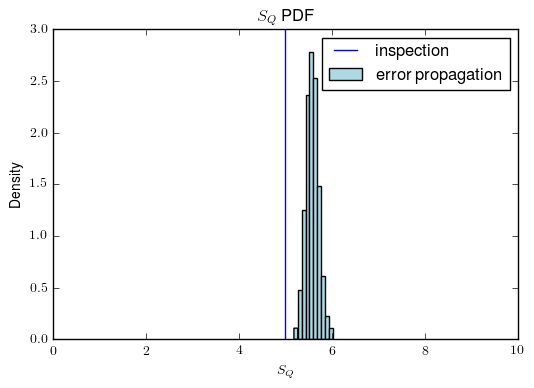
\includegraphics[width=0.6\columnwidth]{error_prop.png}
\caption{
The distribution of conversion factors from error propagation and the conversion factor from visual inspection of the data. 
\label{fig:error_prop}}
\end{figure}

\newpage

\subsection{Re-scaling The Laplace Approximation}
\label{subsec:rescale_la}

When implementing the laplace approximation as described in Subsection \ref{subsec:laplace}, we run into numerical issues.
The large difference in scale between masses and luminosities, differing by as much as $10^{10}$ at times, wipes out the precision in the off-diagonal terms of the Hessian matrix.
This manifests as having zeroes for the off-diagonal elements of the Hessian.
To avoid these issues we run the optimizer over the log mass and log luminosity.
In this section we describe the mathematics that makes this possible.
\\
\noindent Let f represent the log integrand, 

$$f(M,L) = \ln P(L^{obs}|L, \sigma_L^{obs}) + \ln P(L|M, \alpha, S, z) + \ln P(M|z)$$

\noindent Then we use the BFGS algorithm to attain

$$\ln M_{opt}, \ln L^{opt}, H_{ln}^{opt\ -1} = \text{argmin}_{\ln M,\ln L} -\left[f(M,L)\right]$$

\noindent where we optimize over logarithmic mass and luminosity to get an accurate hessian. Then by the chain rule we have 

$$-\frac{\partial^2 f}{\partial M \partial L} = -\frac{\partial^2 f}{\partial \ln M \partial \ln L} \frac{\partial \ln M}{\partial M} \frac{\partial \ln L}{\partial L} = -\frac{1}{ML}\frac{\partial^2 f}{\partial \ln M \partial \ln L}$$

\noindent After extending this to the other combinations of mass and luminosity we have

$$H^{opt} = (H_{ln}}^{opt\ -1})^{-1} \odot \begin{pmatrix}M^{opt}^{-2} & M^{opt}^{-1}L^{opt}^{-1}\\ M^{opt}^{-1}L^{opt}^{-1} & L^{opt}^{-2} \end{pmatrix}$$

\noindent where $\odot$ is elementwise multiplication. Then we can approximate the likelihood as 

$$\mathcal{L}(L^{obs}|\alpha, S, \sigma_L^{obs}, z) = \exp(f(M^{opt}, L^{opt}))\sqrt{\frac{(2\pi)^2}{\det(H^{opt})}}$$

\noindent Now the optimizer provides a Hessian with nonzero off-diagonal entries which produces a much better approximation.


\end{document}
% ======================================================================
% 
